\section{Deep learning}
% something about deep learning 
    % convolutional neural network
        % convolutional layers, pooling, FC
    % maybe about resnet if I wanna compare it
    

Solving mathematical problems is a very easy task for computers. However, the real challenge is to solve problems that are natural to humans but cannot be formally described by a set of rules for computers. Things like understanding spoken words, recognizing objects, or identification of people are all instinctively learned by humans and require years of experience. For computers to gain this knowledge, a similar concept is used. They also learn from experience by using a large amount of provided data. The system of learning is based on a hierarchy of concepts, where each concept is built upon relations with simpler concepts. Drawing a graph of this hierarchy would result in a deep structure of concepts, which is where the name deep learning comes from \cite{Goodfellow-et-al-2016}.

In this section, we will talk about a specific type of deep learning technique - convolutional neural networks. 

\subsection{Convolutional neural network}

A convolutional neural network (CNN) is a specific type of neural network that operates on grid-like data. It is most commonly used when working with images, which are represented as a 2D grid of pixel values \cite{Goodfellow-et-al-2016}.

The process is the same as with a neural network, but the inner structure is different. The CNN receives the input, which is fed through the series of hidden layers and the final score is computed in the output layer. Each layer is made up of a set of neurons, which have learnable weights and biases. However, the neurons in CNN are arranged in 3 dimensions: width, height, and depth as is depicted in the Figure \ref{img:cnn0}.

\begin{figure}[h]
    \centering
    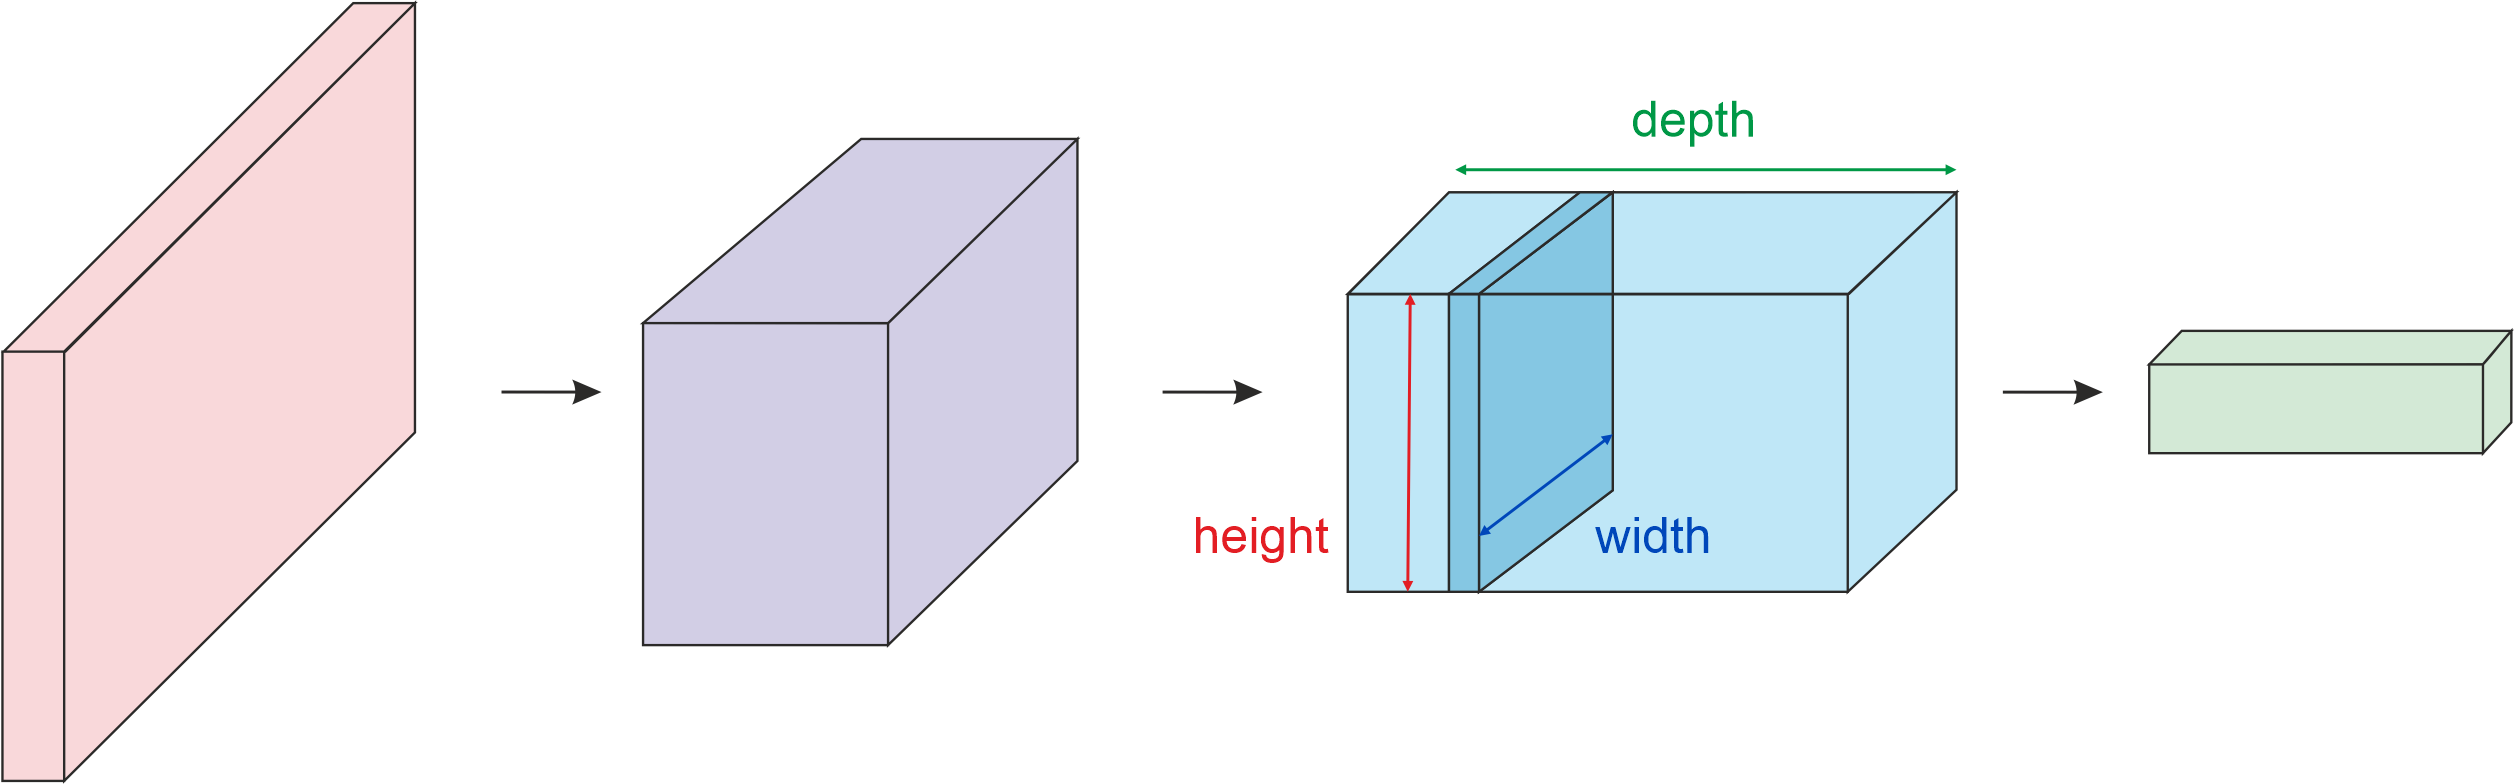
\includegraphics[width=.8\textwidth]{images/cnn.png}
    \caption{Inside structure of convolutional neural network.}
    \label{img:cnn0}
\end{figure}

%In neural networks, layers are fully connected, which means that each neuron from the previous layer is connected to each neuron in the following layer. 

While in neural networks, all layers are fully connected, the CNN has 3 main building blocks: convolutional layer, pooling layer, and fully connected layer \cite{standford}.

\subsubsection{Convolutional layer}

The convolutional layer is the most essential part of CNN and as the name suggests, this is where the convolution operation happens. Each convolutional layer has a defined set of filters/kernels. The filter has a significantly smaller spatial size than the input image (ranging from 3 to 10 pixels wide) but covers the full depth of the input. The values of each filter represent weights learned by the network \cite{standford}.

During the forward pass of the network, the convolution is applied to the input volume in a manner that each filter is moved across the width and height of the input. How many pixels the filter moves during convolution is defined by parameter stride. At each position, a dot product is computed between values of the filter and values of the input. This creates a 2D activation matrix also called a feature map. 
This way, each filter in the layer creates a feature map containing the response of that specific filter at each spatial position of the input. Stacking all these feature maps together builds the output volume of the layer, where the depth is the number of filters in the layer \cite{Goodfellow-et-al-2016} \cite{standford}.

Formally, the convolution is defined by the following formula:
\begin{equation}
    (K * I) (i,j) = \displaystyle\sum_{m}  \displaystyle\sum_{n} I(i - m, j - n) K(m, n).
\end{equation}
where K is the kernel, and I is the input volume \cite{Goodfellow-et-al-2016}.

A simple example of convolution applied to 2D input is shown in the Figure \ref{img:conv0}. It shows how the kernel is moved through the matrix with a stride 1 and how the dot product at each position is calculated. 

\begin{figure}[h]
    \centering
    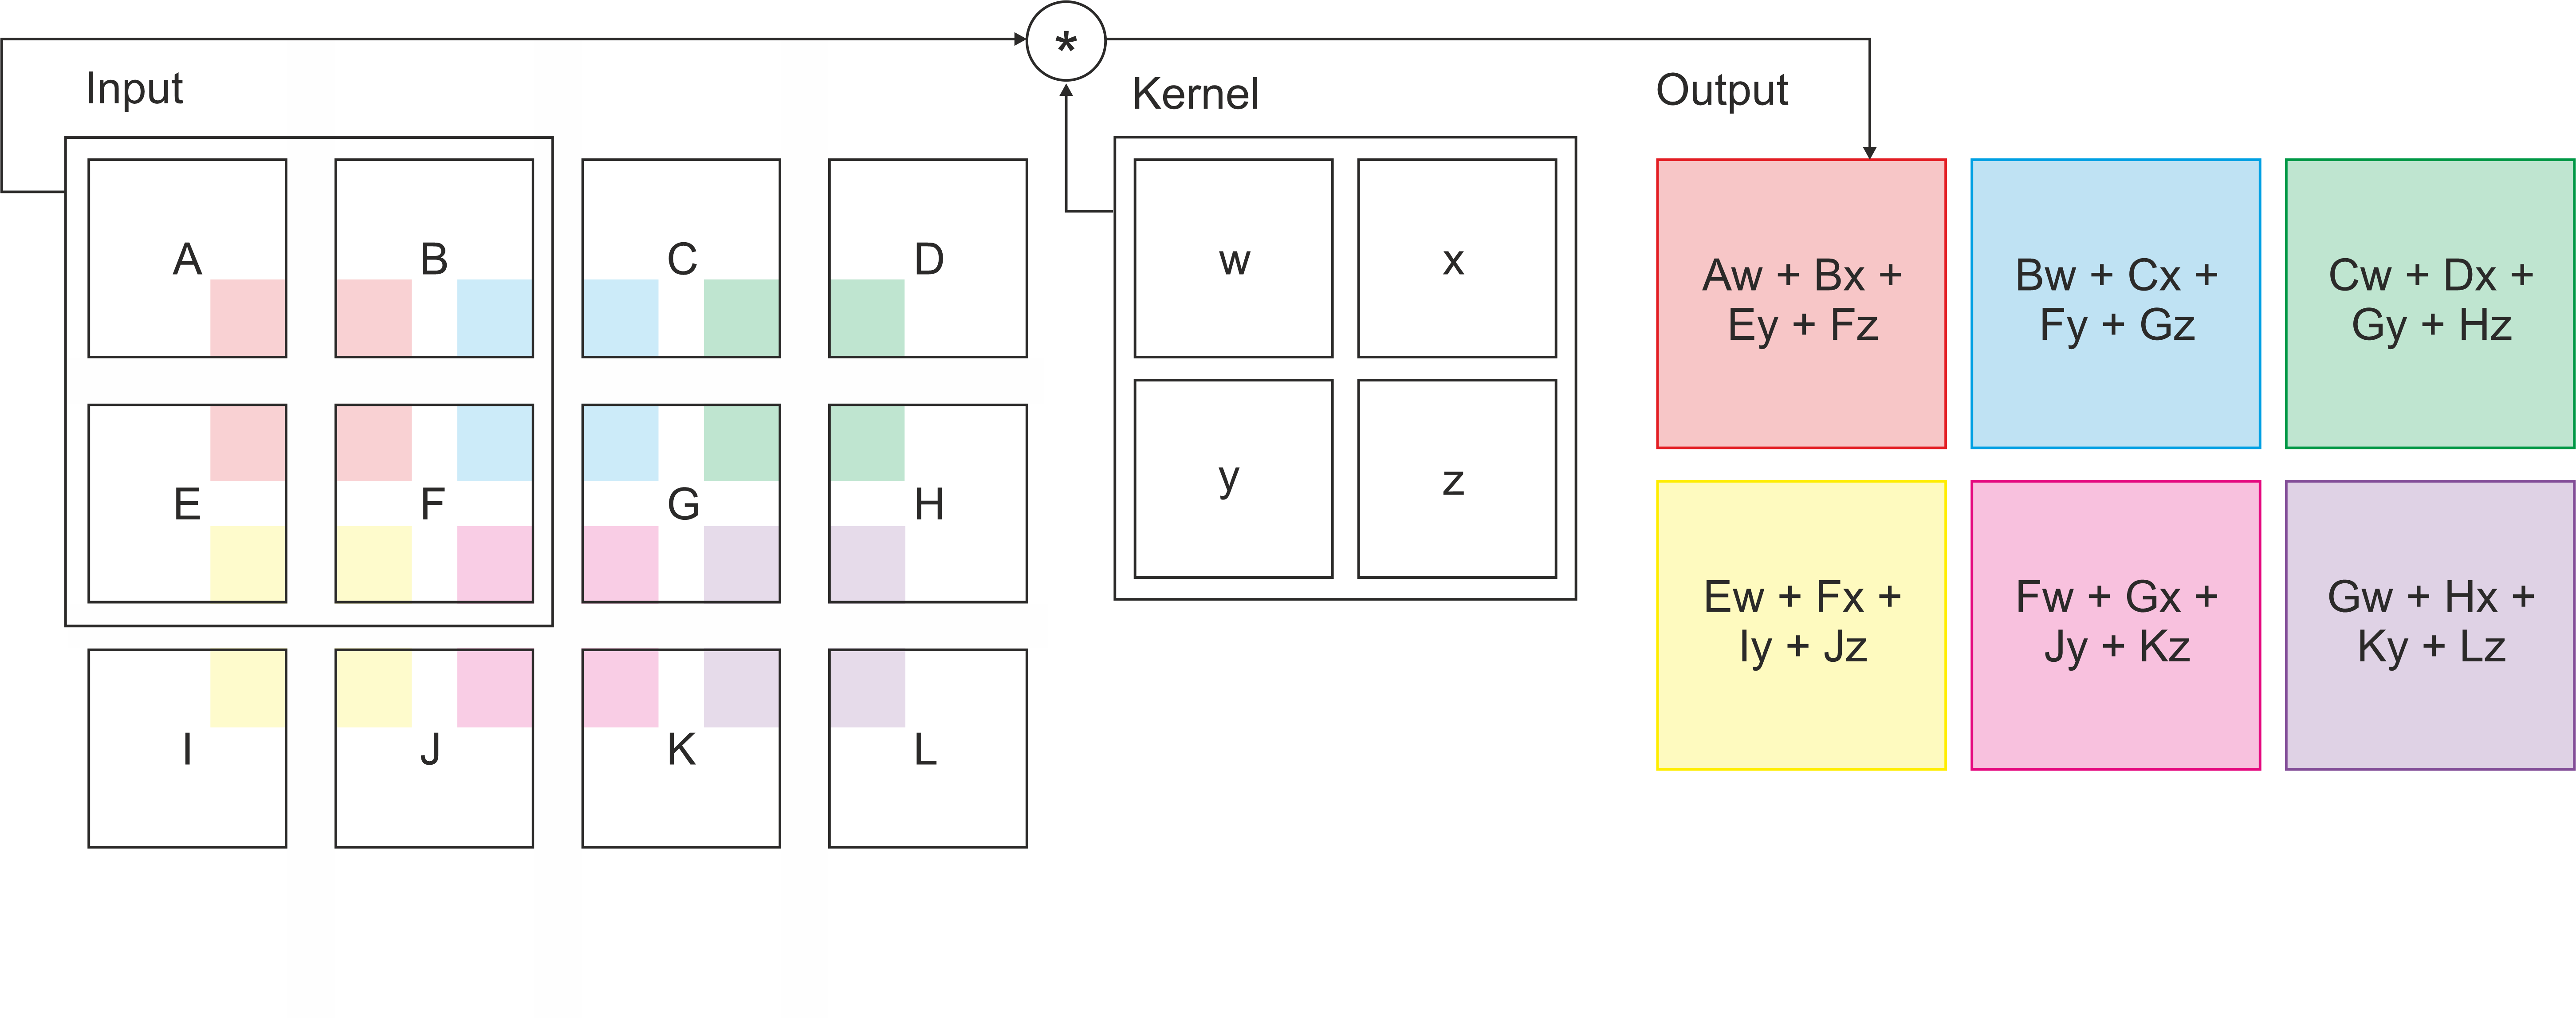
\includegraphics[width=.8\textwidth]{images/convolution3.png}
    \caption{An example of simple convolution.}
    \label{img:conv0}
\end{figure}

\subsubsection{Pooling layer}

Another important layer in the architecture of CNN is the pooling layer. It is useful for reducing the spatial size of feature maps and therefore makes the computation more effective as the network gets deeper. It is also helpful in keeping the representation approximately the same when the input image is slightly translated \cite{Goodfellow-et-al-2016}.

The pooling layer has a defined size of the kernel, which usually ranges from 2x2 to 3x3 pixels spatially. Another important parameter is the pooling function that is performed on the input. The most common is max pooling, but there are other popular pooling functions such as average, weighted average, or L2 norm pooling. 
Unlike other layers in the CNN, the pooling layer has no learnable parameters \cite{standford}.

Pooling is performed in a similar fashion as convolution. A kernel is moved across the input volume spatially but operates on each depth slice separately. This way only the spatial size of the input is reduced and the depth stays the same. At each spatial location, the output value is computed using the pooling function performed on the values of the input \cite{standford}.

The process of max pooling is illustrated in the Figure \ref{img:maxpool0}. The size of the kernel in the example is 2x2 with a stride of 2. It is common practice to use the stride the same size as the kernel if we do not want an overlapping pooling.  

\begin{figure}[h]
    \centering
    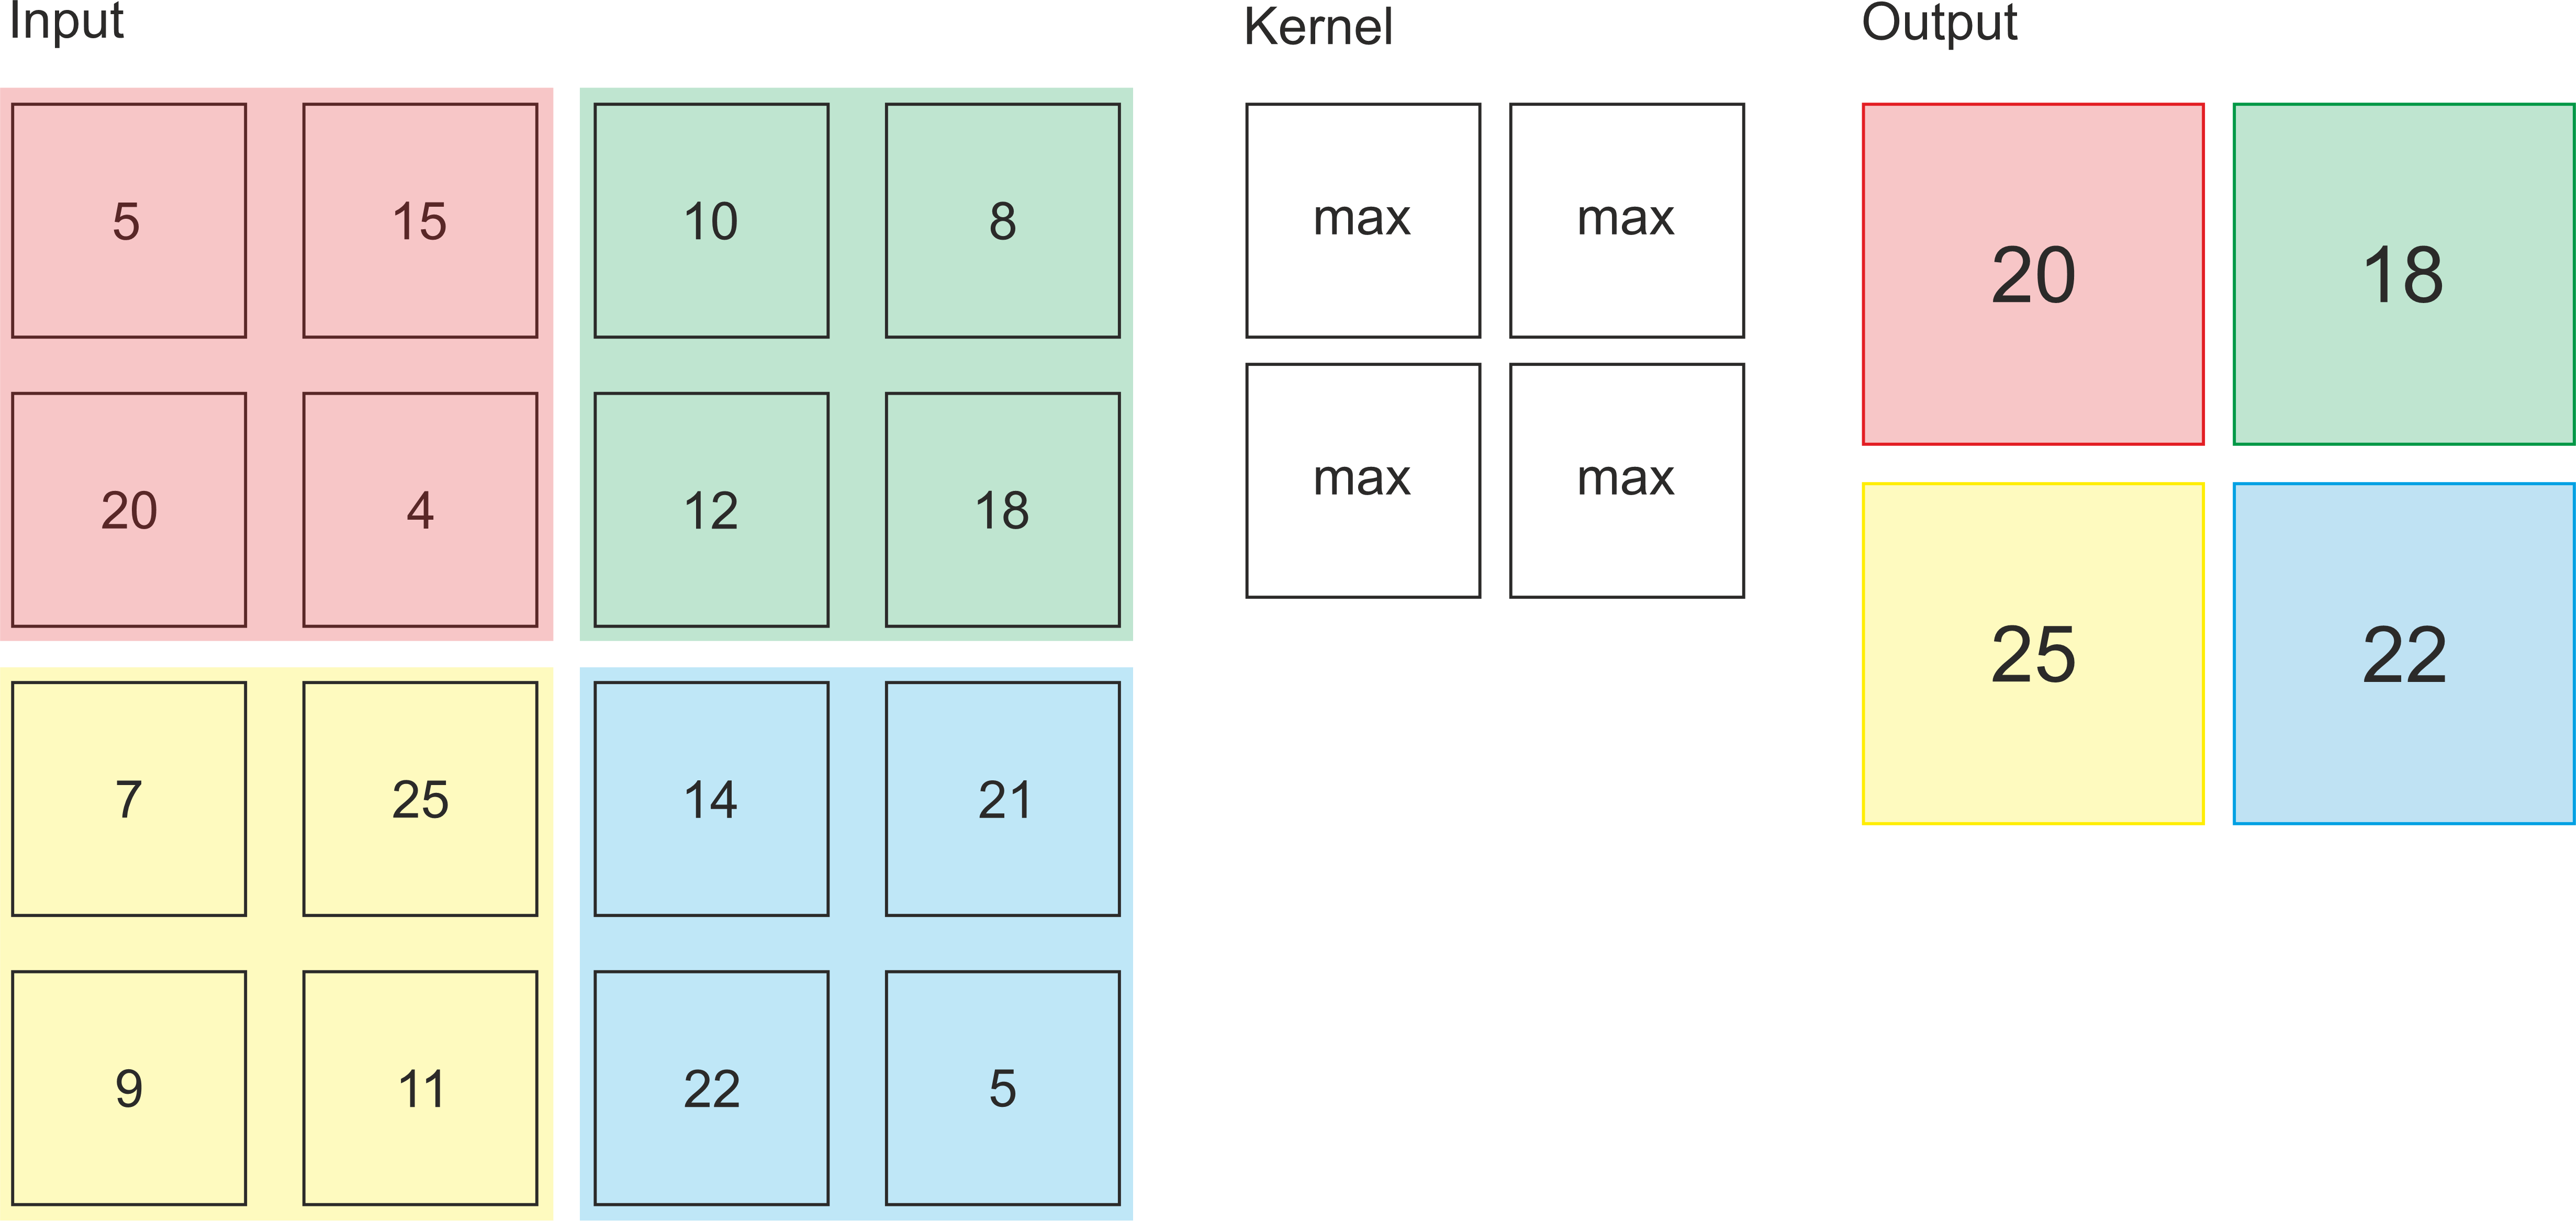
\includegraphics[width=.7\textwidth]{images/maxpooling.png}
    \caption{An example of max pooling.}
    \label{img:maxpool0}
\end{figure}

\subsubsection{Fully-connected layer}
Fully connected (FC) layers in CNN are identical to layers in a standard neural network. They consist of neurons that have no connection to each other within one layer, but each neuron from the previous layer is connected to each neuron in the following layer \cite{Goodfellow-et-al-2016}.

The structure of neurons in FC layers is no longer organized in 3 dimensions instead inputs and outputs are 1D vectors. Feature maps fed to a fully-connected layer, therefore, need to be flattened to one dimension.

While in standard neural networks, each layer is fully-connected, in CNN only the last layers that are responsible for calculating the class scores are fully-connected \cite{standford}.
